\section{Clúster final}
Veient les opcions presentades en les seccions anteriors,  hem decidit escollir la versió que ens dóna més TFlops. Aquesta és la que té nodes dual-socket amb el processador \textit{AMD EPYC 7502}. Hem escollit comprar els commutadors de 40 ports, ja que ens ofereixen el doble de velocitat que els de 36 (200 Gbits i 100 Gbits respectivament).

Podem veure que el percentatge de TFlops de les gràfiques respecte el total és 0.289. Aquest número s'aconsegueix amb 12 GPUs \textit{AMD Radeon Instinc MI50}, posant 6 en dos nodes. Com els nodes tenen 8 slots per gràfiques (PCIe de 16 lanes), podríem afegir 4 targetes gràfiques amb menys TFlops i intentar apropar-nos més al 30\% de TFlops de GPU que ens imposa la restricció.

Per fer-ho, afegim quatre gràfiques \textit{AMD Radeon Pro WX8200}, afegint 2.625 TFlops al nostre clúster. El preu s'incrementa en 3879.96 \$ i el ràtio de \texttt{TFlops GPU/Total} acaba sent 0.296.

Per calcular el consum de potència, hem tingut en compte els següents valors (aproximant aquells dels que no trobàvem dades concretes)
\begin{table}[h!]
\centering
\begin{tabular}{lc}
\hline
\multicolumn{1}{l|}{Component}         & \multicolumn{1}{l}{Consum (W)} \\ \hline
\multicolumn{1}{l|}{\cellcolor[HTML]{EFEFEF}CPUs}        & \multicolumn{1}{l}{\cellcolor[HTML]{EFEFEF}56880}      \\
\multicolumn{1}{l|}{\begin{tabular}[c]{@{}l@{}}GPUs \\ Instinct\end{tabular}} & \multicolumn{1}{l}{3600} \\
\multicolumn{1}{l|}{\cellcolor[HTML]{EFEFEF}\begin{tabular}[c]{@{}l@{}}GPUs \\ Pro\end{tabular}}      & \multicolumn{1}{l}{\cellcolor[HTML]{EFEFEF}920}  \\
\multicolumn{1}{l|}{Memòria \cite{consummem}}     & \multicolumn{1}{l}{3792}       \\
\multicolumn{1}{l|}{\cellcolor[HTML]{EFEFEF}Commutadors \cite{consumnintendo}} & \multicolumn{1}{l}{\cellcolor[HTML]{EFEFEF}500}        \\
\multicolumn{1}{l|}{Total}       & \multicolumn{1}{l}{65692}      \\ \hline
                                  &                                
\end{tabular}
\caption{Càlcul de potència}
\end{table}


\clearpage

Finalment, aquesta és la configuració que hem escollit:
\begin{table}[H]
\begin{adjustwidth}{-1.0in}{-1.0in}
\begin{center}
\begin{tabular}{l|l}
\hline
    {\cellcolor[HTML]{EFEFEF}CPU}         & {\cellcolor[HTML]{EFEFEF}Dual-socket AMD EPYC Rome 7502P \cite{cpu_amd_7502_buy}} \\ 
    Cores/CPU & 32 \\
    \rowcolor[HTML]{EFEFEF}
    Placa base & AMD EPYC 7002 series, dual-socket \cite{dualgpu}\cite{dualnogpu}  \\
Cores/Node                                       & 64                                             \\ 
    {\cellcolor[HTML]{EFEFEF}GPU\_1}                       & {\cellcolor[HTML]{EFEFEF}AMD Radeon Instinct MI50 \cite{gpu_mi50}} \\ 
\#GPU\_1                                           & 12 (2 nodes amb 6 GPUs)                         \\
    {\cellcolor[HTML]{EFEFEF}GPU\_2}                       & {\cellcolor[HTML]{EFEFEF}AMD Radeon Pro WX8200 \cite{gpu_pro_8200}} \\ 
\#GPU\_2                                           & 4 (2 nodes amb 2 GPUs)                         \\
    {\cellcolor[HTML]{EFEFEF}Memòria}     & {\cellcolor[HTML]{EFEFEF}Kingston KSM29RS4 DDR4 2933Hz \cite{mem2}}   \\
{\color[HTML]{000000}Memòries/node}             & {\color[HTML]{000000}8 DIMMS de 16GB}          \\ 
    {\cellcolor[HTML]{EFEFEF}Commutadors} & {\cellcolor[HTML]{EFEFEF}Mellanox MQM8700-HS2F, 200Gbits \cite{mellanox_mqm8700-hs2f}} \\ 
{\color[HTML]{000000}\#Commutadors}             & {\color[HTML]{000000}3}                        \\ 
{\cellcolor[HTML]{EFEFEF}\#Nodes sense GPU (1U)}    & {\cellcolor[HTML]{EFEFEF}77}                       \\
{\color[HTML]{000000}\#Nodes amb GPU (2U)}      & {\color[HTML]{000000}2}                        \\
{\cellcolor[HTML]{EFEFEF}Us de nodes}               & {\cellcolor[HTML]{EFEFEF}81}                       \\
{\color[HTML]{000000}Us de nodes + commutadors} & {\color[HTML]{000000}84}                       \\ \hline
{\cellcolor[HTML]{EFEFEF}TFlops CPU}                & {\cellcolor[HTML]{EFEFEF}197.5}                    \\
{\color[HTML]{000000}TFlops GPU}                & {\color[HTML]{000000}83.085}                    \\ 
{\cellcolor[HTML]{EFEFEF}TFlops Totals}             & {\cellcolor[HTML]{EFEFEF}280.585}                   \\ 
{\color[HTML]{000000}TFlops GPU/Totals}         & {\color[HTML]{000000} 0.296}                    \\ 
{\cellcolor[HTML]{EFEFEF}Cost (Dòllars)}                 & {\cellcolor[HTML]{EFEFEF}1127027.41}              \\
{\color[HTML]{000000}GFlops/Dòllar}               & {\color[HTML]{000000}0.255}                    \\
    \rowcolor[HTML]{EFEFEF}
Power dissipation total (W) & 65692 \\
    Energy efficiency (GFlops/Watt) & 4.374 \\ \hline
\end{tabular}
\caption{Configuració final del clúster.}
\end{center}
\end{adjustwidth}
\end{table}




\subsection{Roofline}


\begin{table}[h]
\begin{adjustwidth}{-1.5in}{-1.5in}
\begin{center}
\begin{tabular}{l||c|c|c}
    \hline
Component                           & \multicolumn{2}{c|}{Specifications}                                         & Bandwith (GB/s)          \\ \hline  \hline 
                                    & \cellcolor[HTML]{EFEFEF}bits/T               & \cellcolor[HTML]{EFEFEF}64  &                          \\
                                    & GT/s                                         & 2.922851563                 &                          \\
    \multirow{-3}{*}{DRAM}              & \cellcolor[HTML]{EFEFEF}Channels             & \cellcolor[HTML]{EFEFEF}8   & \multirow{-3}{*}{187.06} \\ \hline
                                    & GT/s                                         & 2.922851563                 &                          \\
                                    & \cellcolor[HTML]{EFEFEF}Effective trans bits & \cellcolor[HTML]{EFEFEF}32  &                          \\
    \multirow{-3}{*}{Infinity fabric 2} & Directions                                   & 2                           & \multirow{-3}{*}{23.38}  \\ \hline
                                    & \cellcolor[HTML]{EFEFEF}Lanes                & \cellcolor[HTML]{EFEFEF}128 &                          \\
\multirow{-2}{*}{PCIe 4.0}          & GT/s                                         & 16                          & \multirow{-2}{*}{256.00} \\ \hline
\multirow{-1}{*}{Hbm2 amd mi50} & \cellcolor[HTML]{EFEFEF}- & \cellcolor[HTML]{EFEFEF}- & 1024.00 \\ \hline
\multirow{-1}{*}{Hbm2 amd pro} & - & - & 512.00 \\ \hline
\end{tabular}
    \caption{Bandwidth de cada element de transmissió de dades del socket.}
    \label{tab:peak_bw}
\end{center}
\end{adjustwidth}
\end{table}

A la taula \ref{tab:peak_bw} observem quin és el bandwidth màxim que podem obtenir amb cada component del socket, el qual és el mateix pel node. Hem tingut en compte l'accés a memòria a través dels canals de memòria i a través de d'Infinity Fabric 2 \cite{amd_if2}, el xip d'interconnexió equivalent al QPI d'Intel. També hem calculat l'accés per PCIe perquè es necessari per enviar/rebre les dades a/de la memòria de la targeta gràfica.

\begin{table}[h]
\begin{adjustwidth}{-1.5in}{-1.5in}
\begin{center}
\begin{tabular}{c||c|c|c}
    \hline
Component                                                                            & \multicolumn{2}{c|}{Specs}                                         & GFlops                     \\ \hline \hline
                                                                                     & \cellcolor[HTML]{EFEFEF}Freq (GHz)  & \cellcolor[HTML]{EFEFEF}2.5 &                            \\
                                                                                     & ops/cycle                           & 16                          &                            \\
\multirow{-3}{*}{\begin{tabular}[c]{@{}l@{}}AMD EPYC\\ 7502P\end{tabular}}           & \cellcolor[HTML]{EFEFEF}\#cores     & \cellcolor[HTML]{EFEFEF}32  & \multirow{-3}{*}{1280}     \\ \hline
                                                                                     & FP64 GFlops                         & 6865.92                     &                            \\
\multirow{-2}{*}{\begin{tabular}[c]{@{}l@{}}AMD Radeon\\ Instinct Mi50\end{tabular}} & \cellcolor[HTML]{EFEFEF}GPUs/socket & \cellcolor[HTML]{EFEFEF}3   & \multirow{-2}{*}{20597.76} \\ \hline
                                                                                     & FP64 GFlops                         & 672                         &                            \\
\multirow{-2}{*}{\begin{tabular}[c]{@{}l@{}}AMD Radeon\\ Pro WX8200\end{tabular}}    & \cellcolor[HTML]{EFEFEF}GPUs/socket & \cellcolor[HTML]{EFEFEF}1   & \multirow{-2}{*}{672}      \\ \hline
\end{tabular}
    \caption{GFlops per cada component de càlcul d'un socket.}
    \label{tab:gflops_socket}
\end{center}
\end{adjustwidth}
\end{table}

A la taula \ref{tab:gflops_socket} hem calculat els GFlops que ens aportaria un processador, 3 targetes gràfiques AMD Radeon Instinct MI50 i 1 AMD Radeon PRO WX8200, ja que són els elements de càlcul d'un socket. Per tant, ara toca desglosar el càlcul del peak bandwidth i performance en funció del tipus de node: d'1 U, només amb CPUs, i de 2 U, amb CPUs i GPUs.

\subsubsection{Només CPU}
En el nostre clúster un dels tipus de node que tenim és només amb processadors. Procedim a calcular el peak bandwidth i performance per socket i node:

\begin{itemize}
    \item Socket:
        \begin{itemize}
            \item Peak bandwidth
                \[187.06\ GB/s\ DRAM + 23.38\ GB/s\ IF2 = 210.45 GB/s\ socket\]
            \item Peak performance
        \[ 1\ CPU \times 1280\ GFlops/cpu = 1280\ GFlops\ socket\]
        \end{itemize}
    \item Node:
        \begin{itemize}
            \item Peak bandwidth
                \[210.45\ GB/s\ socket = 210.45\ GB/s\ node\]
            \item Peak performance
\[2\ sockets \times 1280\ GFlops/socket = 2560\ GFlops/node\]
        \end{itemize}
\end{itemize}

\begin{figure}[H]
    \centering
    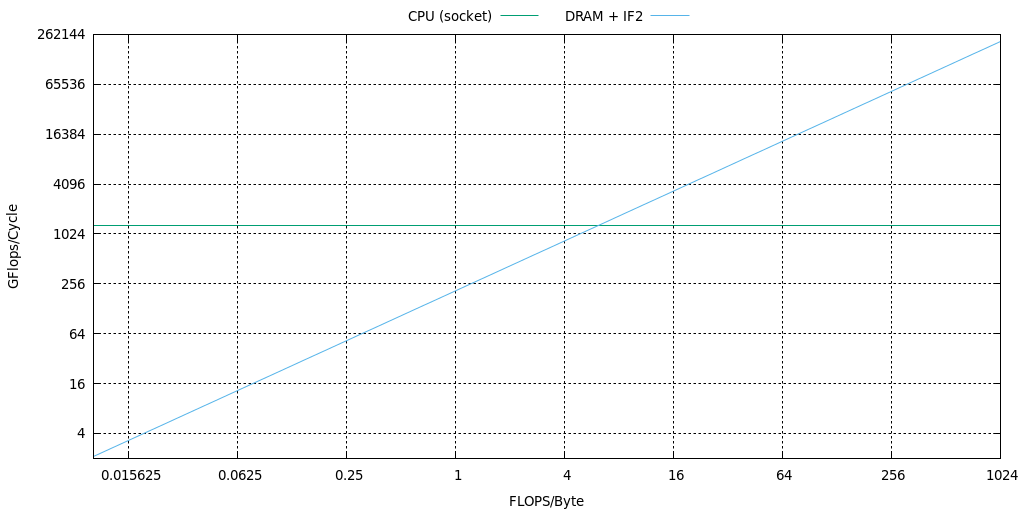
\includegraphics[width=\textwidth]{entregable/img/roofline_cpus_dram}
    \caption{Model Roofline amb només CPUs en un socket}
    \label{fig:summary}
\end{figure}

\begin{figure}[H]
    \centering
    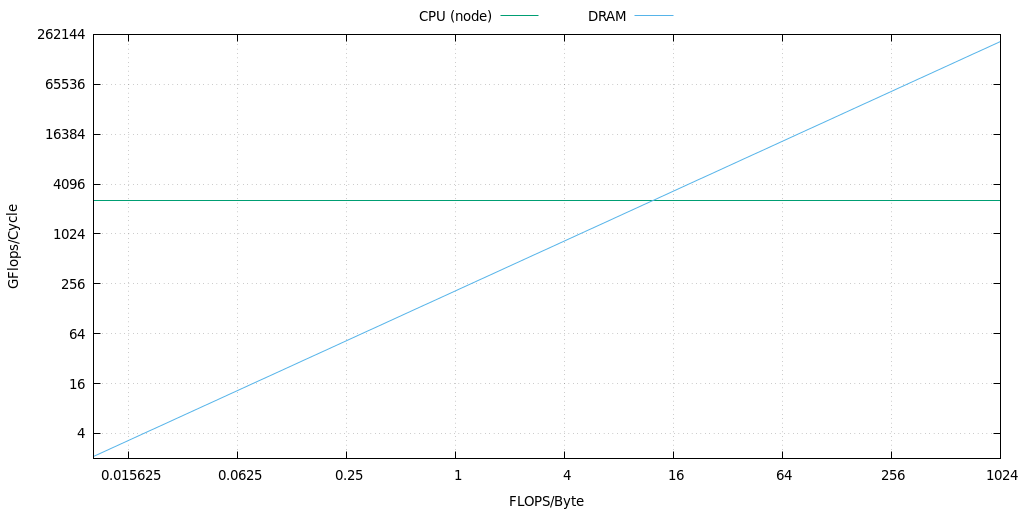
\includegraphics[width=\textwidth]{entregable/img/roofline_cpun_dram}
    \caption{Model Roofline amb només CPUs en un node}
    \label{fig:summary}
\end{figure}

\subsubsection{Només GPU}

\begin{itemize}
    \item Socket:
        \begin{itemize}
            \item Peak bandwidth
                \[3\ MI50 \time 1024\ GB/s\ HDM2 + 1\ WX8200 \time 512\ GB/s\ HBM2 = 3584 GB/s\ socket\]
            \item Peak performance
                \[3\ MI50 \time 20597.76\ GFlops/MI50 + 1\ WX8200 \time 672\ GFlops/WX8200 = 692.12 TB/s\ socket\]
        \end{itemize}
    \item Node:
        \begin{itemize}
            \item Peak bandwidth
                \[2\ sockets \times 3584\ GB/s\ socket = 7168\ GB/s\ node\]
            \item Peak performance
\[2\ sockets \times 692.12\ TFlops/socket = 1384.23\ GFlops/node\]
        \end{itemize}
\end{itemize}


\begin{figure}[H]
    \centering
    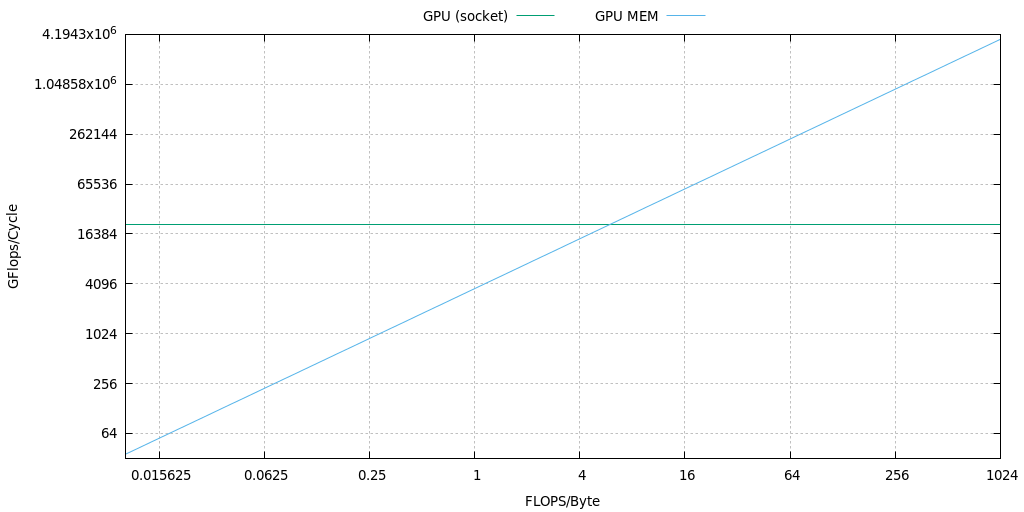
\includegraphics[width=\textwidth]{entregable/img/roofline_gpus_memgpu}
    \caption{Model Roofline amb només GPUs en un socket}
    \label{fig:summary}
\end{figure}

\begin{figure}[H]
    \centering
    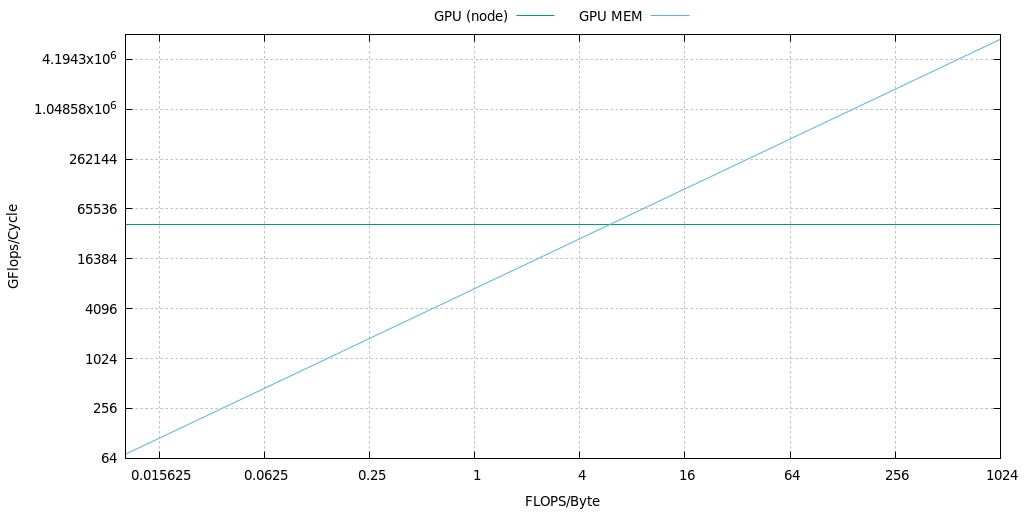
\includegraphics[width=\textwidth]{entregable/img/roofline_gpun_memgpu}
    \caption{Model Roofline amb només GPUs en un node}
    \label{fig:summary}
\end{figure}

%    \item GFlops socket node 2U:\\
%        \[ \begin{aligned} 1280\ GFlops/cpu + 20597.76\ GFlops/GPU\_MI50 + \\ + 672\ GFlops/GPU_WX8200 = 1280\ GFlops/socket \end{aligned} \]
%
%    \item GFlops node 2U:\\
%\[2\ sockets \times 1280\ GFlops/socket = 2560\ GFlops/node\]
%\end{itemize}
